\chapter{Overview}
\index{overview}

\package{} handles the following three basic tasks: importing,
validating, and exporting papers. We discuss these briefly below and
return to discuss each of them in the following chapters.

\section{Importing Papers}

When importing a list of papers, they end up in a publication
database stored as a simple text file. The file is stored in the
current working directory and is named \emp{papers.pub}. When new data is
imported into the database, both the database and the imported data
are validated. The two lists of papers are subsequently merged (with
check for duplicates) and stored back to the database, as illustrated
in Figure~\ref{fig:import}.

For more details, see Chapter~\ref{import}.

\begin{figure}[htbp]
  \begin{center}
    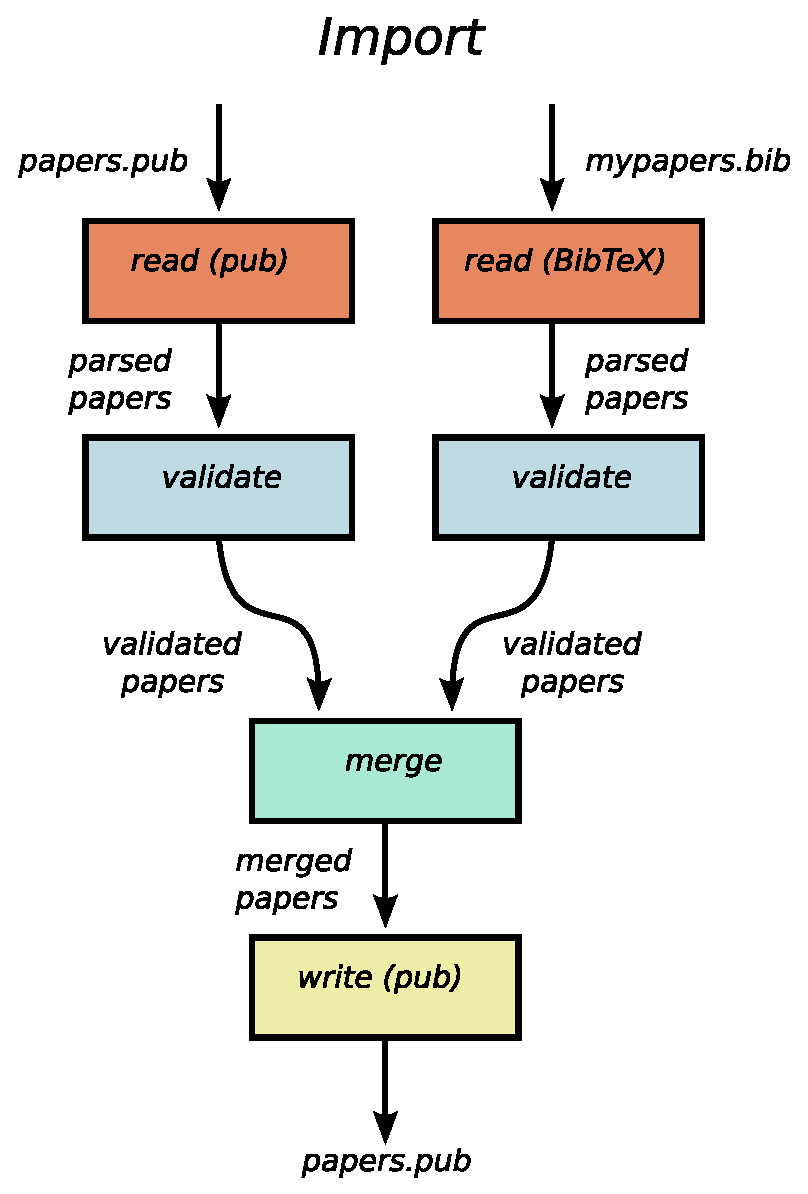
\includegraphics[width=12cm]{images/import.eps}
    \caption{Importing papers.}
    \label{fig:import}
  \end{center}
\end{figure}

\section{Validating Papers}

After data has been imported into the database, it is possible to
validate the database for errors. Validation happens automatically
when data is imported, so this feature is mostly relevant when the
database file is edited directly. A schematic overview of the
validation process is given in Figure~\ref{fig:validate}.

For more details, see Chapter~\ref{validate}.

\begin{figure}[htbp]
  \begin{center}
    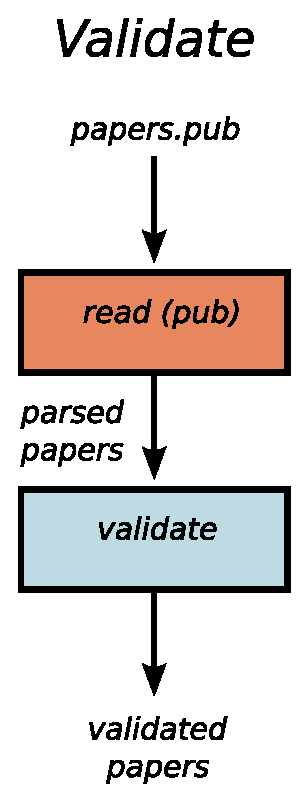
\includegraphics[width=4cm]{images/validate.eps}
    \caption{Validating papers.}
    \label{fig:validate}
  \end{center}
\end{figure}

\section{Exporting Papers}

Publication records may be exported from the database in one of the
following formats: \emp{pub}, BibTeX, \LaTeX, or PDF. The
user may also specify a filter to export a subset of the papers in the
database, for example all papers in a specific category or from a
specific year.  During export, all papers are first read from the
database, then validated, then filtered, and then formatted, as
illustrated in Figure~\ref{fig:export}.

For more details, see Chapter~\ref{export}.

\begin{figure}[htbp]
  \begin{center}
    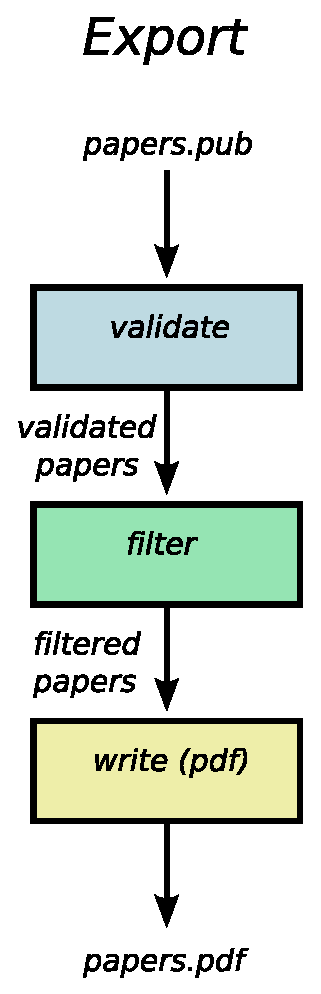
\includegraphics[width=4cm]{images/export.eps}
    \caption{Exporting papers.}
    \label{fig:export}
  \end{center}
\end{figure}

\section{The \texttt{pub} Format}
\index{pub-format}

The system uses its own format for storage of the papers. The format
is designed to allow simple editing\footnote{The format is based on
the Emacs Org-Mode. Database files may thus be conveniently edited
using the Org-Mode, see Appendix~\ref{orgmode}.}  and looks as
follows:

\begin{code}
* category
** title
   attribute: value
   attribute: value
   ...
** title
   attribute: value
   attribute: value
   ...
* category
   ...
\end{code}

See Appendix \ref{pubformat} for more information about the
\texttt{pub} format.

The papers imported into the system will end up in one of 12 categories, see
Table~\ref{tab:categories}. When exported to PDF or
HTML\footnote{HTML-output is not implemented in version 1.0}, they will
be put under the matching headline.

\begin{table}[htbp]
  \begin{center}
    \begin{tabular}{|l|l|}
      \hline
      \textbf{Category} & \textbf{Headline}\\
      \hline
      \hline
      articles & Articles in International Journals\\
      books & Books\\
      edited & Edited Books\\
      chapters & Chapters in Books\\
      refproceedings & Refereed Proceedings\\
      proceedings & Conference Proceedings\\
      reports & Technical Reports\\
      manuals & Manuals\\
      theses & Theses\\
      courses & Courses\\
      talks & Talks\\
      misc & Other Publications\\
      \hline
    \end{tabular}
    \caption{Paper categories and headlines.}
    \label{tab:categories}
  \end{center}
\end{table}

Which category is assigned to a paper depends on what BibTeX
entry-type\index{BibTeX entry-type} the paper has, or, alternatively,
the category specified by the user when importing papers.

\begin{table}[htbp]
  \begin{center}
    \begin{tabular}{|l|l|}
      \hline
      \textbf{Category} & \textbf{BibTeX entry-type}\\
      \hline
      \hline
      articles & article\\
      books & book\\
      edited & book, proceedings\\
      chapters & inbook\\
      proceedings & inproceedings, conference\\
      reports & techreport\\
      manuals & manual\\
      theses & phdthesis, mastersthesis\\
      courses, talks, misc & misc\\
      not supported & booklet, incollection, unpublished\\
      \hline
    \end{tabular}
    \caption{Paper categories and corresponding BibTeX entry-types.}
    \label{tab:entrytypes}
  \end{center}
\end{table}

As can be seen in table \ref{tab:entrytypes}, some categories match
several entry-types, and some entry-types match several categories.
\package{} implements some simple rules to deduce which category
should be assigned to any given paper with known BibTeX
entry-type. This is discussed in more detail in
Chapter~\ref{import}.
